\documentclass[10pt]{article}


\usepackage{wrapfig}
\usepackage{float}
\usepackage{graphicx}
\usepackage{amsmath,amsthm,amssymb,comment}
\usepackage[noend]{algpseudocode}

\usepackage[left=0.5in,right=2in]{geometry} 
\usepackage[textwidth=1.5in]{todonotes}

\DeclareMathOperator*{\argmax}{arg\,max}
\DeclareMathOperator*{\val}{val}

% \usepackage[noend]{algpseudocode}
% \usepackage{algorithm}
% \usepackage{algorithmicx}

\newcommand{\R}{\mathbb{R}}
\newcommand{\N}{\mathbb{N}}
\newcommand{\Z}{\mathbb{Z}}

\newtheorem{definition}{Definition}
\newtheorem{lemma}{Lemma}
\newtheorem{theorem}{Theorem}
\newtheorem{conjecture}{Conjecture}

\begin{document}

% \renewcommand{\qedsymbol}{\filledbox}

\title{
  You Can't Handle the Lie: \\
  Next-Hop Verification in BGP
}
\author{
  Clay Thomas\\ claytont@cs.princeton.edu
  \and 
  Gavriel Hirsch\\ gbhirsch@cs.princeton.edu 
}
\maketitle

\begin{abstract}
  This paper presents a new protocol called \emph{Next-Hop Verification},
  which that reduces the set of contexts in which
  other autonomous systems are incentivized to lie while participating in BGP.
  The protocol works by sharing information about BGP path announcements
  between different ASs, using the existing structure of the network,
  and checking those path announcements against the true flow of traffic
  in the data plane.
  We discuss the advantages and disadvantages of this new approach,
  and compare its effectiveness to that of previously considered verification
  techniques.
\end{abstract}


\section{Introduction}

  \subsection{Background and Previous Work}
    Routing on the Internet involves many distinct Autonomous Systems (AS's), each
    with its own data sources, destinations, and links; as well as its own
    preferences over how traffic is routed. An AS may prefer that the traffic it
    sends and receives be sent over the shortest path, in order to decrease
    latency; or it may prefer to send its traffic through or avoiding specific
    other AS's for economic incentives, due to contracts between AS's about
    routing costs; or it may prefer to avoid certain other AS's, if it is
    concerned about malicious activity. In the other direction, an AS may also
    prefer to attract or deter traffic from certain other AS's, again for economic
    incentives or perhaps even to spy on certain traffic.

    These AS's typically use the Border Gateway Protocol (BGP) to announce
    routes to neighbors and learn routes from neighbors in the control plane,
    and to then choose how to actually route traffic in the data plane. However,
    there is no way for BGP to enforce the requirement that an AS route traffic in a
    way that matches its announcements.
    Thus, due to all of the various (often conflicting)
    preferences that AS's have over how traffic is routed, these
    AS's can often have incentives to lie in the control plane about what they
    will actually do in the data plane, in order to influence how other AS's behave.

    To counteract this, \emph{verification protocols} have been developed which
    run alongside or alter BGP in order to prevent lying.
    Unfortunately, directly verifying the routes a packet takes in the data plane
    requires cryptographic signatures on every packet, as in \cite{DataPlane}.
    This huge overhead makes full data-plane verification impractical.
    Instead, previous work has searched for control plane protocols
    which still manage to prevent or discourage certain types of lies.

    Much work has been done on analyzing BGP verification protocols
    through game-theoretic models.
    \cite{RoutingGames} shows that in a general set of contexts, a form of
    verification called \emph{path verification}\footnote{
      In the original
      paper they refer to it as route verification.}
    ensures that no AS or group of
    AS's can get strictly preferred routes for its traffic by telling lies.

    However, lying can potentially give other benefits beyond getting better
    routes for your own traffic.
    \cite{Attraction} analyzes BGP games in which agent's utility may depend
    on attracting traffic from other AS's.
    In this scenario, even using path verification does not suffice to
    disincentivize lying.
    They introduce another form of verification
    called \emph{loop verification}, which is simpler but weaker, and describe
    conditions under which path or loop verification do disincentivize lying.
    However, they admit that many of these conditions are unreasonably strong,
    such as requiring that AS's always announce either all paths they are aware
    of or none at all to all of their neighbors.
    
    Another proposal for detecting BGP lies---or more generally BGP faults---is NetReview \cite{NetReview}. When using NetReview, AS's record and publish all their BGP messages in tamper-evident logs, and other AS's are able to audit these logs to check whether there are any faults. However, actually detecting the faults requires regularly auditing the entirety of every AS's logs which is nontrivial. In addition, NetReview is purely in the control plane, so additional work needs to be done if we are concerned that AS's may route in the data plane differently than what they announced in the control plane. Next-hop verification addresses both of these concerns by being relatively simpler, and by incorporating information from the data plane.

  \subsection{Our contributions}
    Given the difficulty of preventing lies in BGP,
    we would at least like to be able to \emph{detect} lies when they are told.
    The initial observation of this work is that
    there will always be at least one AS that knows what each
    other AS is truly doing, namely the one that directly receives traffic from
    it in the data plane.
    As a result, if AS's are willing to collaborate then there is
    information that can be used to detect the existence of lies, without
    requiring full data-plane verification. Put another way, we can just monitor
    each AS, rather than every packet.
    Based on this observation, we present a new protocol called
    \emph{next-hop verification}
    and show that it effectively prevents lies in certain scenarios.

    As with previous practical verification protocols,
    next-hop verification protocol runs in the control plane.
    However, it also uses
    information sampled from the data plane in order to aid verification.
    Specifically, it requires AS's to keep track of which of its neighbors
    forward traffic towards it for different destinations.
    Given that agents have this information, next-hop verification gives an
    effective way for agents to distribute queries and fact-checking
    using the existing structure of the network and no encryption.

    We find that assuming full compliance, next-hop verification allows us to catch lies assuming
    there are is no traffic attraction among preferences.
    In this regard, next-hop verification is similar in effectiveness to 
    path verification.
    In the context where preferences involve traffic attraction,
    we are able to significantly weaken the assumptions which
    \cite{Attraction} needed on the preferences of AS's.
    In this sense, next-hop verification is sometimes more powerful
    than path verification (although there do exist cases where
    path verification will prevent a lie that next-hop verification cannot).
    Additionally, we find that next-hop verification is strictly more
    powerful than loop verification, that is, every lying situation detected
    by loop verification will be detected by next-hop verification
    (though loop verification is still more lightweight).
    In general, we attempt to embark on a similar program to that of
    \cite{Attraction}, experimenting with various settings and seeing
    where next-hop verification leads to good incentive properties.

\begin{comment}
  \subsection{Organization}
    \todo{Might not need this in a ``workshop style paper''}
    In the rest of Section 1 we discuss existing work, and we briefly outline
    our results and their limitations. Section 2 informally presents the model
    we use. Section 3 describes the next-hop verification protocol. Section 4
    states and proves some theorems about the implications of using next-hop
    verification, and goes through examples of concrete scenarios to compare
    what would be possible with and without next-hop verification. Finally,
    Section 5 offers some suggestions for follow-up work and Section 6 concludes.
\end{comment}


\section{Model Details}
  \subsection{BGP framework}
    We model the network of AS's as an undirected graph, with a node for each AS
    and an edge between any two AS's that can directly communicate with each other
    without going through a third AS. We assume that the graph is a single
    connected component, so any AS can in theory interact with any other AS.
    As is standard in the literature, we assume there is a unique destination AS
    $d$, because routing to different destination (prefixes) is done
    independently in BGP.

    In the BGP framework, AS's can announce the
    existence or removal of paths to each other.
    Each AS has an import policy that
    determines how it responds to path announcements from neighboring AS's.
    Specifically, the import policy determines whether the AS will update
    its route, given a new announcement.

    Each AS also has an export policy which determines how it will communicate the
    paths it is aware of to other AS's.
    Specifically, for a BGP compliant AS, the export policy determines
    whether or not to announce the AS's currently chosen route to a given neighbor.
    In realistic settings an AS may prefer not to announce its path to all neighbors
    (the most famous example of this being \cite{GaoRexford},
    in which for example customers will not route traffic
    between two of their providers).
    However, for a manipulative, non-BGP compliant AS,
    a much richer set of export policies is available.
    The AS can lie arbitrarily, announcing paths that it doesn't use
    or that don't even exist.

    Finally, each AS has some preferences over how the actual traffic in the
    network flows. The AS's will choose a strategy, namely their import and export
    policies, based on these preferences.

    \begin{definition}
      Suppose a BGP network $G$ has reached a stable equilibrium.
      We say that an AS \textbf{m} is \textbf{lying} if the
      it exports a route other than that which it is using.
      We say that an AS is \textbf{honest} if it is not lying.
    \end{definition}
    
    We assume that the collection of strategies leads the network to converge to a
    stable solution.
    In general contexts, convergence becomes very hard to
    reason about. Because of this complexity and the fact that in practice convergence does occur,
    in this paper we choose to focus on what happens after
    convergence. We show that if the network were to converge to a state that
    depends on lies, we would then be able to catch the lies and shame the liar.
    As a result, it should not be beneficial to lie in a way that leads to that
    state.
    If you are interested in the topic of convergence though, see
    \cite{RoutingGames, Attraction, StablePaths, PolicyPathVector}
    for examples of more formal details about proving different types of convergence
    and what assumptions are necessary.


  \subsection{Verification}
    In this section, we give an overview of some previously considered 
    verification protocols. These will be our comparison points for next-hop
    verification.

    \begin{definition} 
      In a network using \textbf{path verification} it is
      impossible for AS's to announce that they are using paths which were not
      already announced to them.
    \end{definition}

    Some extensions to BGP, such as S-BGP, can enforce path verification.
    However, it requires additional overhead as well as universal adoption
    \cite{PartialDeploy}, because every route communicated in the control plane
    must be cryptographically signed by every AS along that route.

    \begin{definition}
      In a network using \textbf{loop verification} no AS will
      use an export policy that involves not sending a path to a neighbor
      specifically because that neighbor is already in the path.
      In addition, if
      an AS ever sees a path containing itself that it did not announce, it will
      ``raise an alarm'', with the idea that the offender (the first
      node which announced a false path) can be publicly shamed.
    \end{definition}

    Note that if instead export policies did not send paths to neighbors who are
    already in them, the alarming in loop verification could not always be done.

  \subsection{Behavioral assumptions}
    When agents get utility from attracting traffic, stronger verification
    protocols are needed to disincentivize lying.
    In \cite{Attraction}, the authors consider the following classes of
    preferences which depend on more than just an AS's own path.

    \begin{definition}
      An AS $m$ cares about \textbf{volume attraction} if its utility can depend on
      the set of AS's that route through $m$.
      
      An AS $m$ cares about \textbf{generic attraction} if its utility can depend on
      the set of AS's that route through $m$ AND on the routes these AS's take to get to $m$.
      \end{definition}

    Volume attraction can reflect truly malicious situations such as spying,
    where the manipulative agent wants to view packets for some nefarious
    reason. Issues like this may occasionally have huge consequences for the
    global routing behavior of the internet, for example, the 2010
    China Telecom BGP hijacking could've potentially served this function
    \cite{ChinaHijack}. It could also simply reflect an economic incentive such as
    getting paid for routing more traffic.
    
    With preferences for generic attraction, an AS $m$ may have incentives to affect
    \emph{how} other agents route through $m$.
    For example, a provider may want a customer to route directly through it
    in order to charge that customer more.

    We briefly consider one assumption on the path preferences of AS's as well:
    \begin{definition}
      An AS $n$ has a \textbf{next hop policy} if its utility for a given path
      is a function of only the first AS along the path (i.e. the next-hop).
    \end{definition}

\section{Next-Hop Verification Protocol}
  % Once convergence has occurred, we propose the use of the following protocol by
  % all of the AS's. Note that the malicious AS $m$ may lie and not follow the
  % protocol in order to avoid being caught, but since convergence has already
  % occurred we assume that none of the other AS's have an incentive to lie or even
  % to hide information they know.
  We now define next-hop verification.
  This protocol is run on a BGP network after convergence has already occurred.
  Nodes communicate along existing links in the network, storing and sending
  next-hop queries. We assume that AS's can ``raise the alarm'', similar to
  \cite{Attraction}, which refers to alerting others that something
  is going wrong with the particular query. For our results section,
  we will assume that when the alarm is raised, the offending agent will be
  caught (for example, via the collaboration of the NANOG mailing list to detect
  the problem, as suggested in \cite{Attraction}).

  Each node maintains a queue of queries which it needs to answer.
  A query is denoted $Q_d(a,b)$, representing a node announcing that
  $a$ uses $b$ as its next-hop in its path to destination $d$.
  During initialization, every node $n$ adds the query $Q_d(a,b)$ to its own
  queue, for every hop $(a,b)$ on $n$'s path to the destination $d$.
  From that point on, every round in which $n$ acts, it runs the function
  {\sc Respond} on every query $Q_d(a,b)$ waiting in its queue, then waits for more queries.

  \begin{algorithmic}[1]
    \State Denote the acting AS by $n$
    % \Function{Initialize}{}
    %   \For {each hop $(a,b)$ in $n$'s path to $d$}
    %     \State Add the query $Q_d(a,b)$ to your query queue
    %   \EndFor
    % \EndFunction
    \Function{Respond}{$Q_d(a,b)$}
      \If { $n$ previously responded to $Q_d(a,b)$ }
        \State \Return
      \EndIf
      \If { $n = a$ }
        \If { $n$ does not use $b$ as its next hop for $d$ }
          \State ``raise the alarm'' \label{line:sourceRaise}
        \EndIf
        \State \Return
      \EndIf
      \If { $n = b$ }
        \If { $a$ does not use $n$ as its next hop for $d$ }
          \State``raise the alarm'' \label{line:targetRaise}
        \Else
          \State send the query $Q_d(a,b)$ to all neighbors
            \label{line:falseNegativeForward}
        \EndIf
        % \State send the query $Q_d(a,b)$ to all neighbors
      \Else \ (i.e. $n \neq a,b$)
        \If {$a$ uses $n$ as its next hop for $d$ }
          \State ``raise the alarm'' \label{line:otherRaise}
        \Else
          \State send the query $Q_d(a,b)$ to all neighbors
            \label{line:cluelessForward}
        \EndIf
      \EndIf
    \EndFunction
    % \SetKwFunction{Respond}{Respond}
    % \Function{Main}{}
    %   \For {each query $Q_d(a,b)$ in $queue$}
    %     \State {\sc Respond}($Q_d(a,b)$)
    %   \EndFor
    %   \State clear the $queue$
    % \EndFunction

  \end{algorithmic}

  \subsection{Additional considerations}
  \begin{itemize}
    \item In the case where $n$ is responding to a query $Q_d(a,n)$, it needs to
      check whether $a$ actually forwards traffic directly to $n$ for
      destination $d$, which must be done in the data plane. Accordingly, each
      AS should keep a flag for each other (neighboring AS) $\times$ (dest AS)
      pair, representing whether the first AS ever directly sends $n$ traffic
      destined for the second $AS$.
    \item In practice, maintaining the accuracy of this information in the
      face of the dynamic nature of routing would be difficult.
      However, we take this information as given.
      In particular, we assume that traffic is sent often enough toward the
      destination that the absence of traffic means that a given route is not
      being used. \todo{rephrase}
    % \item If an AS has too many neighbors and/or destinations and keeping all
    %   these flags becomes unmanageable, each AS can have a policy for
    %   determining which pairs it thinks are important to monitor for.
    %   \todo{idk if the previous bullet should encompass this??}
    \item If a manipulator is lying about the next-hop it is personally using,
      it may intentionally send occasional traffic towards its announced
      next-hop, while sending the bulk of its traffic down the route that it
      genuinely prefers. We take this strategy into consideration, and our
      theorems hold even allowing for this. However, it means that next-hop
      verification cannot ``confirm the hop'' if $n=b$ and $a$ uses $b$ as
      its next-hop, and must instead forward the query on to its neighbors
      in line~\ref{line:falseNegativeForward} of {\sc Respond}.
      ((WE HAVE A CONCRETE EXAMPLE OF THIS IF THERE IS SPACE,
      AT LEAST FOR VOLUME ATTRACTION))
  \end{itemize}

  For a motivating example of next-hop verification, consider the
  network given in Figure~\ref{fig:Nonexistent}.
  Here, $m$ is able to get a preferred path to the destination by falsely
  announcing the path $md$ to node $2$.
  However, nodes $1$ and $d$, which are both one hop away from $2$,
  can tell that this announcement is not legitimate:
  $d$ knows that $m$ does not route directly to $d$,
  and $1$ knows that $m$ routes directly to $1$ instead of $d$.
  Thus, both $d$ and $1$ will ``raise the alarm'' if they are compliantly
  running next-hop verification.
  \begin{figure}[h]
    \centering
    \caption{NonexistentPath}\label{fig:Nonexistent}
    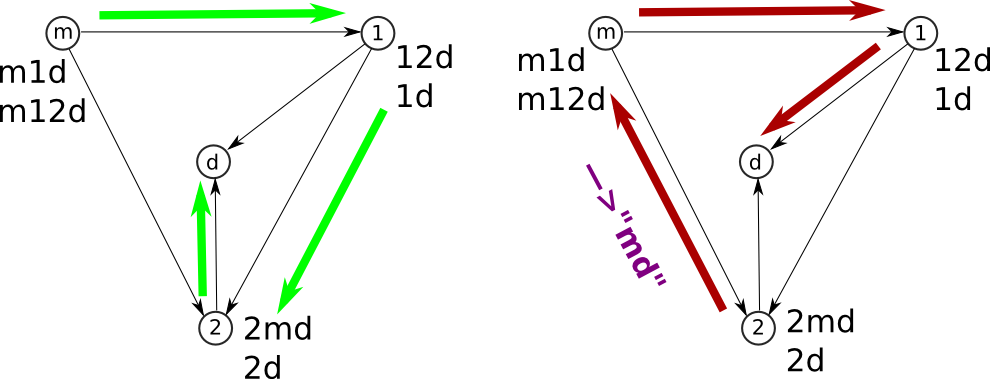
\includegraphics[width=0.75\textwidth]{NonexistentBetter}
  \end{figure}

\section{Results}

  % The following lemma is the key to our positive results.
  % It explains whey next-hop verification
  % \begin{lemma}
  %   Let $G$ be a BGP instance with the next-hop verification phase.
  %   Suppose all nodes except one manipulator $m$ are next-hop participants.
  %   Assume that $m$ announces to node $v$ a hop $(a,b)$, where in the data plane the
  %   hop $(a,c)$ is used for some $b\ne c$.
  %   (Note that both $b$ and $c$ may be used if $a=m$ and $m$ is ``faking traffic'').
  %   Furthermore, suppose there exists a path from $v$ to $c$ not containing $m$.
  %   Then $m$ with be caught by next-hop verification, and will
  %   receive utility $-\infty$.
  % \end{lemma}
  % \begin{proof}
  %   Let $P$ denote the path from $v$ to $c$ not containing $m$.
  %   Because the activation sequence is fair, every node along the path with
  %   be activated, in the proper order going from $v$ to $c$.
  %   % \todo{
  %   %   Note: should probably get rid of the protocol's ability to
  %   %   ``drop queries'' in view of a false-negative
  %   % }
  %   Node $v$ starts with the query $Q(a,b)$, and thus it will eventually travel
  %   to $b$, which will ``raise the alarm'' and give $m$ utility $-\infty$.
  % \end{proof}

  Our first result formalizes the statement ``in a network without
  traffic attraction, next-hop verification will catch all incentivized lies''.
  Figure~\ref{fig:Nonexistent} demonstrates this theorem, as discussed above.
  \begin{theorem}
    Let $G$ be a stable outcome of a BGP instance without traffic attraction.
    Suppose there is a single manipulator $m$,
    and all other nodes honestly participate in BGP and in next-hop verification.
    If $m$ lies in order to get a better path to $d$,
    then next-hop verification will catch that lie and shame $m$.
  \end{theorem}
  \begin{proof}
    Suppose $m$ announces a hop $(a,b)$ to $v$, where $(a,c)$ is actually in
    a route from $m$ to $d$ for some $c\ne a$.
    (Note that $m$ could send traffic to both $b$ and $c$ if $m=a$.)
    For contradiction, assume that every path from $c$ to $v$ includes $m$
    % (so $m$ can drop the next-hop queries and its lie won't be caught).
    The route from $m$ to $d$ which includes $(a,c)$ must not have loops, so it cannot include $m$ again.
    If there was a path from $v$ to $d$ which did not contain $m$, then the
    path from $c$ to $d$ would give a simple path from $v$ to $c$ not containing
    $m$. Thus, every route from $v$ to $d$ includes $m$.

    Because all non-$m$ nodes are honest, $m$ must get $v$ to change its route
    to $d$ in order to get a different path by lying to $v$.
    (More technically, there must exists a choice of
    $v$ which picks a different path).
    However, $v$'s route cannot effect $m$'s route to $d$, because
    every route from $v$ to $d$ includes $m$,
    so no route of $v$ nor any consequence of $v$'s route can change the set of
    paths available to $m$.
    This contradicts the assumption that $m$ got a better path by lying,
    and shows that there exists a path $P$ from $c$ to $v$ not including $m$.

    Now, because all nodes along $P$ are participating in the next-hop protocol,
    the node $v$ will ask the query $Q_d(a,b)$, which will travel along path $P$
    until $c$ can ``raise the alarm'' in line~\ref{line:otherRaise} of {\sc
    Respond}.
  \end{proof}

  The next result shows that next-hop verification is at least as
  powerful as loop verification:
  \begin{theorem}
    Let $G$ be a stable outcome of a BGP instance.
    Suppose there is a single manipulator $m$ who lies in the stable outcome,
    and all other nodes honestly participate in BGP and in next-hop verification.
    Then if $m$ would be necessarily be caught by loop verification,
    % were used by all other nodes,
    then $m$ will be caught by next-hop verification.
  \end{theorem}
  \begin{proof}
    As shown above, an AS cannot be incentivized to lie just to get a better
    path: there must be traffic attraction.
    Suppose $m$ attracts traffic from some node $v$ by falsely announcing a path
    $P$ from $m$ to $d$.
    The manipulator $m$ must announce the path $P$, paths containing $P$
    must spread outward through some part of the graph, and $v$ must end up
    routing through $P$.
    Let the tree of agents who end up routing through $P$ be denoted by $T$
    (in particular, $v\in T$). Note that $T\setminus \{m\}$ is connected.

    % Consider all the AS's that this announcement travels
    % through to get to $v$. These AS's form a path $Q$ from $m$ to $v$. Note
    % that, because all non-$m$ nodes are honest, all the nodes in $Q$ must still
    % have the path containing $P$ installed in the final stable outcome.
    % ((NOTE: MAYBE Q SHOULD BE A TREE INSTEAD OF A PATH))

    Now, the only way for loop verification to guarantee to be able to
    catch $m$ in this lie is if some
    node $q$ in the tree $T$ is adjacent to a node $u$, such that $P$ contains
    the path $uR$, where $R$ is a route that $u$ did not announce. Indeed,
    in this case a route containing $P$ can be announced to $u$ by $q$,
    and $u$ can raise the alarm for loop verification.

    Let $(a,b)$ be the first hop along $R$ which is not actually used in the
    data plane. Note that $m\notin R$.
    If next-hop verification is used by all non-manipulator nodes, then $v$ will
    ask the query $Q_d(a,b)$. This query will travel within the tree $T$,
    through $q$ to $u$, and along $R$ until it gets to $a$.
    There, agent $a$ will ``raise the alarm'' in line~\ref{line:sourceRaise} of {\sc
    Respond}, and $m$ will be caught.
  \end{proof}
  As an aside, we note that an analogue of the above theorem for path
  verification does not hold\footnote{
    For an example, consider figure~\ref{fig:Bowtie}, altered by removing the
    link between nodes $m$ and $l$. The exact same lying strategy is still
    available to $m$ under next-hop verification, but this is not possible if
    path verification is used.
  }.
  Combined with the extensive discussion in \cite{Attraction},
  the previous result gives us a few different situations in which
  next-hop verification will catch all incentivized lies.
  The rest of this section is dedicated to weakening the requirements
  for those incentive-compatibility properties to hold.

  The following theorem says that next-hop verification will still catch lies
  in networks with volume attraction.
  Indeed, unlike \cite{Attraction} we do not need to make \emph{any} assumptions
  on preferences or behavior (other than assuming \emph{volume} attraction)
  to get this positive result.
  \begin{theorem}
    Let $G$ be a stable outcome of a BGP instance with traffic volume attraction.
    Suppose there is a single manipulator $m$,
    and all other nodes honestly participate in BGP and in next-hop verification.
    If $m$ lies in order to attract traffic from some node $u$,
    then next-hop verification will catch that lie and shame $m$.
  \end{theorem}
  \begin{proof}
    % As shown before, $m$ cannot get a better path. We show further
    % that $m$ cannot attract more traffic (in volume).
    Suppose $m$ did manage to attract more traffic from a victim $u$.
    Let $P$ denotes the path $u$ originally took to $d$,
    and let $Q$ denote the path $u$ takes in the manipulated outcome $G$.
    Note that $m\in Q$ but $m\notin P$.
    Let $v$ denote a node that $m$ lied to, and suppose $v$ is told
    that hop $(a,b)$ is used while $(a,c)$ is actually used for $c\ne b$.

    Because the lie told to $v$ must effect the path chosen by $u$,
    there exists a path $R$ from $u$ to $v$ not including $m$.
    Furthermore, because $m$ uses the route $S$ from $c$ to $d$
    (and profits from it) we know $m\notin S$.
    Thus, by eliminating any possible loops from $RPS$,
    the concatenation of the three paths,
    we get a simple path from $v$ to $c$ which does not include $m$.
    Because all non-$m$ nodes are actively and honestly running next-hop,
    the query $Q_d(a,b)$ will travel from $v$ to $c$ and $c$ will
    ``raise the alarm'' in line~\ref{line:otherRaise} of {\sc
    Respond}.
  \end{proof}

  However, we are not able to extend this result to generic attraction.
  Indeed, consider the example given by (Figure~\ref{fig:Bowtie}),
  from \cite{Attraction}.
  In this network, the manipulator $m$ wants nodes $n$ and $c$
  to use $m$ as their next hop for destination $d$,
  for example, because of economic considerations.
  The AS's who know what $m$ is doing in the data plane
  are separated from the AS's $m$ is lying to.
  Those victim agents cannot communicate with $d$ and $l$ without
  going through $m$, which can just throw their next-hop queries away
  to avoid being caught.
  \begin{figure}[h]
    \centering
    \caption{Bowtie}\label{fig:Bowtie}
    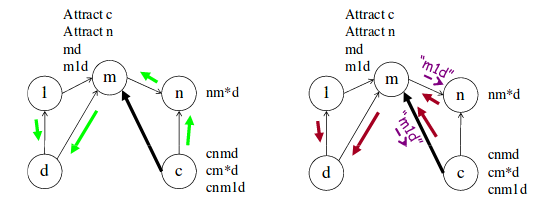
\includegraphics[width=0.75\textwidth]{Bowtie}
  \end{figure}

  We note also that next-hop verification is able to catch the manipulator in
  many of the examples from \cite{Attraction} (indeed, next-hop verification
  works for all examples except Bowtie and DisputedPath).
  This may hint at many more theorems that we were unable to prove for this
  project. In particular, we make the following conjecture:
  \begin{conjecture}
    Let $G$ be a stable outcome of a BGP instance with generic traffic attraction.
    Suppose there is a single manipulator $m$,
    and all other nodes honestly participate in BGP and in next-hop verification.
    Furthermore, assume all nodes use next-hop policy in ranking their paths.
    If $m$ lies in order to attract traffic from some node $u$,
    then next-hop verification will catch that lie and shame $m$.
  \end{conjecture}
  Intuitively, this should eliminate examples like Bowtie, where the victim node
  $c$ was tricked into routing directly through $m$ because his policy was not
  next-hop.
  % ((NOTE: the right assumption in the above might be some sort of ``next-hop
  % attraction'', which sounds similar to AT4 from Goldberg. However, discussing AT4 
  % takes us way too far down the Gao-Rexford rabbit hole)).


\section{Possible future directions}

  \todo{I shortened several of these paragraphs.
  Let me know if I was too heavy-handed!}

  We showed in the previous section that next-hop verification has the potential
  to provide some major benefits for catching lies in BGP, and thus reducing or
  even eliminating AS's incentives to do so. However, there is still some future
  work that should be done before it is used in practice.

  One important question is how effective the protocol can be in partial
  deployment or participation. In our theorems we assumed that there was only
  one malicious AS and that all others actively participated fully in helping to
  catch lies. However in practice, it maybe the case that some AS's have not
  deployed the necessary software and/or hardware for participation.
  Partial deployment and participation would still be somewhat valuable:
  certainly lies can still be detected if we get lucky and all the right agents
  participate. However, a formal analysis with strong theorems is probably
  difficult in the face of such partial deployment.

  A related and interesting line of investigation would be into the
  actual incentives of mutual participation in next-hop verification.
  There are examples where a non-lying agent does actually get a better path
  through the lies of a manipulator, AND that agent's participation is needed to
  catch the manipulator with next-hop verification.
  \todo{check this!!!!}
  In practice, perhaps could ``fact-checking'' be written into
  customer-provider contract agreements,
  e.g. providers helping customers keep track of \emph{other} providers?
  In the setting of Gao-Rexford networks \cite{GaoRexford}, it may be possible
  to prove strong results, such as participation in next-hop with your customers
  never being harmful.

  % It may also
  % be the case that some AS's choose not to participate or to only share a
  % limited subset of the information they have, even if they are not themselves
  % malicious, lying agents.

  %  While this would not give us the same degree of
  % benefits as full participation, it would still allow for the sharing of some
  % information and thus preventing some lies. That said, it would be worth doing
  % a more formal analysis of what this would look like.

  Perhaps the biggest practical problem with our protocol
  is the way it ``floods'' the AS graph with next-hop queries.
  In practice, the very minimum that would need to be added is a
  ``time to live'' field on the next-hop queries,
  which would prevent them from exploding over the entire AS graph.
  % {Somewhat relatedly}, our protocol uses an unencrypted ``flooding'' sort of
  % approach to send queries through the network to their desired recipients. As
  % we saw in Figure~\ref{fig:Bowtie} though, if there is a bottleneck where all
  % paths between two particular nodes goes through a malicious AS, it may want to
  % read the queries that pass through it and drop ones that could expose it. More
  % generally, in a situation with only partial deployment or with multiple
  % malicious AS's, this problem could become more severe, cutting off AS's that
  % both want to fact-check each other.

  The clear alternative to this ``query flooding'' is to simply encrypt the
  query and send it to the AS's who can answer it (just as you would normal traffic).
  The burden of such encryption would not be very heavy, and the
  resulting protocol would be a lot more practical for checking on hops which
  are far away from you in the AS graph.
  \todo{
    the rest of this paragraph is what I meant in that mystery bullet point
    in the google doc
  }
  However, the ideal fact-checking protocol is one that makes only local
  communication, like that of path verification (with local cryptographic signatures)
  or the even more lightweight loop verification (which is normal BGP with a simple
  extra check for ``did I actually announce this?'').
  Indeed, in examples like Figure~\ref{fig:Nonexistent}, the next-hop query
  needs to travel only one hop before being answered.
  In today's very dense AS graph, that may often be the case,
  and with more refined knowledge of the nearby structure of the graph,
  an AS may be able to intelligently route its next-hop queries to get efficient
  answers. We view our protocol, and the theorems surrounding it, as a step
  towards a more refined next-hop verification capable of meeting these
  criterion.

  % next-hop verification is ever deployed in practice, we think it is important
  % to consider this and other tradeoffs between keeping it as simple as possible,
  % and keeping it as secure as possible.

  % One possible way to resolve this would be to add encryption so that an
  % intercepting AS cannot read the query. Or if there are concerns about the AS
  % even knowing whether a query has been sent, the query could even be routed as
  % though it was just normal traffic.

  % We see a possible value in using this sort of approach, but we also see
  % benefits in the unencrypted ``flooding'' approach.
  % The biggest problem we see
  % with this alternative approach is that it makes it more complicated for AS's
  % to adopt and deploy systems that can do next-hop verification, since it would
  % require cryptographic techniques that they AS's may not already be using. If
  % next-hop verification is ever deployed in practice, we think it is important
  % to consider this and other tradeoffs between keeping it as simple as possible,
  % and keeping it as secure as possible.


\section{Conclusion}
In this paper we have proposed the design of Next-Hop Verification, a protocol for catching BGP lies by using information from the control plane along with minimal data from the data plane, and by having the AS's collaborate with each other to detect these lies. We also analyzed the theoretical capabilities of the protocol, and showed that in many circumstances it is capable of catching lies that loop verification and path verification cannot catch. We believe that Next-Hop Verification's approach of sharing informationand cross-checking with the data plane is a valuable one, and that the protocol is a valuable step in working toward more secure control-plane communication.

\todo{Put a code appendix I guess?? As per piazza. At minimum we need to link
to the code}

\bibliography{proj}{}
\bibliographystyle{alpha}

\clearpage

\end{document}
